
\section{Solr}

\subsection{Installation}

Als Systemvoraussetzungen ist eine Java Version $> 8$ gegeben. Ich habe mich hierbei für OpenJDK 11 entschieden. 
Nach dem ersten Starten wurden 2 Warnungen gemeldet, dass die User-Limits für Solr zu gering sind \ref{lst:warningSolr}. Nachdem beide entsprechend erhöht wurden, verschwanden die Warnungen.

Um Solr im Entwicklermodus auszuführen, kann das entpackte Programm einfach mit \path{bin/solr start} gestartet werden. 

\begin{lstlisting}[language=bash, frame=single, label={lst:warningSolr}] 
    *** [WARN] *** Your open file limit is currently 1024.
    It should be set to 65000 to avoid operational disruption.

    *** [WARN] ***  Your Max Processes Limit is currently 63918.
    It should be set to 65000 to avoid operational disruption.
\end{lstlisting}

Die richtige Installation installiert Solr als Service und legt sich einen eignen Nutzer an. Ein entsprechendes Installations-Skript findet sich dafür im entpackten Solr-Ordner.

\subsection{Indexierung}

Um mit der Indexierung starten zu können, muss zuerst in sogenannter „Core“ erstellt werden. Dieser ist ein Index mit dazugehörigen Transaktionslog und Konfigurationsdateien. Nur mit diesen ist es möglich Dateien zu indexieren und auf ihnen zu suchen. Nach der Erstellung lässt sich der Core nun auch über die Oberfläche einsehen und zum Teil konfigurieren.

Damit Solr nun die Daten von der Datenbank liest, muss ein DataImportHandler (DIH) \ref{lst:dih} geschrieben werden. In diesen werden die Daten, welche Indexiert werden sollen mit MySQL-Queries eingelesen. Das System basiert dabei auf Entitys. Diese besizten jedeweils mehre Attribute, wie den Name, welcher auf der Oberfläche zur Indexierung angezeigt wird, den MySQL-Query mit dem die Daten gelesen werden und einen Delta-Query, welcher nur die neuen Einträge lädt. Der Delta-Query benötigt hierbei eine eigene Timestamp-Spalte in der Datenbank, welche angezeigt, wann die Spalte das letzte mal editiert worden ist. Da die Tabellen im Projekt eine solche Spalte nicht besitzen können die Delta-Querys nicht getestet werden. Innerhalb des Entity Elements gibt es entweder weitere Entitys, dazu gleich mehr, oder Field-Elemente. Diese besitzen ein Attribut, welches die Spalte der Tabelle ausweist und einen Namen, der das zugehörige Solr-Schema-Element ausweist. 
Entitys können unbegrenzt ineinander verschachtelt werden. Damit Änderungen an einer verschachtelten Entity nach oben richtig weitergegeben werden, gibt es ParentDeltaQuerys. Diese geben die betroffenen Werte an die übergeordnete Entity weiter. Dafür führt der ParentDeltaQuery einen Aufruf an die überliegende Entity-Tabelle aus in der er mithilfe der Femdschlüssel-Ids in den betroffen Zeilen herausfindet.

Der DataImportHandler muss, bevor er benutzt werden kann, jedoch noch mit dem Core verbunden werden, dafür wird er, zusammen mit einem JDBC-Treiber in die solrconfig.xml eingetragen. Bei den JDBC-Treiber habe ich mich bei diesem Beispiel für den Treiber von MariaDB entschieden. Damit es nicht deswegen zu Laufzeit-Unterschieden bei der Indexierung kommen kann, werde ich diesen Treiber bei allen Systeme mit JDBC-DataImportHandlern verwenden.

\begin{lstlisting}[language=xml, frame=single, label={lst:dih}, 
    morekeywords={entity,query,deltaQuery,parentDeltaQuery,field,column, name}] 
    <entity name="lemma" 
      query="select * from lemma" 
      deltaQuery="select eid from lemma 
        where last_modified > '${dataimporter.last_index_time}'"> 
		<field column="bezeichnung" name="bezeichnung" />
    [...]
    <entity name="lemma_gnd" 
      query="select * from lemma_gnd where fk_lemma='${lemma.id}'"
      deltaQuery="select * from lemma_gnd 
        where last_modified > '${dataimporter.last_index_time}'"
      parentDeltaQuery="select * from lemma 
        where id=${lemma_gnd.fk_lemma}">
			
        <entity name="gnd" 
          query="select * from gnd where id = '${lemma_gnd.fk_gnd}'"
          deltaQuery="select * from gnd 
            where last_modified > '${dataimporter.last_index_time}'"
          parentDeltaQuery="select * from lemma_gnd where fk_gnd=${gnd.id}">
          <field column="nummer" name="gnd_nummer" />
          <field column="schlagwort" name="gnd_schlagword" />
          [...]
        </entity>
      </entity>  
    </entity>
\end{lstlisting}

Wie schon eben angesprochen, muss das Solr-Schema für die entsprechende Elemente auch angepasst werden. Dieses Schema dient dazu die Dateitypen für eine möglichst gute Indexierung auszuweisen. Dafür wird zuerst der Dateityp für die Tabellen-Spalte angegeben. Dabei werden bei den Grundtypen, zum Beispiel unter anderem String und $text_de$ gelistet. Ohne genauer darüber nachzudenken, habe ich angenommen, dass beide gleichwertig sind und nur für spätere Abfragen auf Sprachen eine Relevanz besitzen. Als ich allerdings eine Abfrage stellte, die alle Lemmata mit den Buchstaben S finden sollte, bekam ich mehr Ergebnisse als erwartet. Dies liegt daran, dass $text_de$, das Feld aus Volltext ausweißt. Deswegen wird jedes Wort als einzelne Entity gewertet und so kamen Lemma, in welchen irgendein Wort mit S begann in meine Auflistung. Auch muss darauf geachtet werden, ob man String oder Strings als Typen angibt, letzteres weist das Feld als multiValued aus, bildet also eine 1 zu N Beziehung ab. So kann man zusammen mit der Verschachtelung N zu M Beziehungen abbilden. Genaueres zu diesem Thema allerdings in Kapitel !!Kapitel anfügen!!.
Um diese Einträge auszuweisen gibt es mehrere Möglichkeiten. In diesem Fall habe ich die Einträge über die Administrations-Oberfläche angelegt. Es ist allerdings auch möglich eine eigenen Shema-Datei zu erstellen. Diese Methode soll allerdings nicht mehr verwendet werden, da es die Möglichkeit gibt, diese Einträge per API einlesen zu lassen. Dabei wird direkt überprüft, ob die Einträge formal stimmen. So können keine fehlerhaften Schemata gebaut werden. Die Einträge, welcher über die API oder die Administrations-Oberfläche gestellt werden, werden in einer Datei names $managed_schema$ im XML-Format angelegt \ref{lst:managedSchema}.


\begin{lstlisting}[language=xml, frame=single, label={lst:managedSchema}, 
    morekeywords={type,uninvertible,indexed,stored,field,multiValued, name}] 

    [...]
    <field name="ddc_webdewey_is_checked" type="boolean" 
        uninvertible="false" indexed="true" stored="true"/>
    <field name="description" type="text_de" uninvertible="false" 
        multiValued="true" indexed="true" stored="true"/>
    <field name="erweiterung" type="text_de" 
        uninvertible="false" indexed="true" stored="true"/>
    [...]

\end{lstlisting}

Die Indexierung lief eine Minute und 34 Sekunden für run 14 Tausend Einträge \ref{img:solrIndexTime}. Dabei wurde der gegebene Arbeitsspeicher nicht komplett ausgenutzt, was darauf schließen lässt, dass die Datenbank der limitierende Faktor war. Die hohe Anzahl der Abfragen ist darauf zurückzuführen, dass Solr keine Joins verwendet, sondern bei jeder verschachtelten Entity die gesammte Tabellen nach passenden Einträgen durchsucht.

\begin{figure}
	\centering
	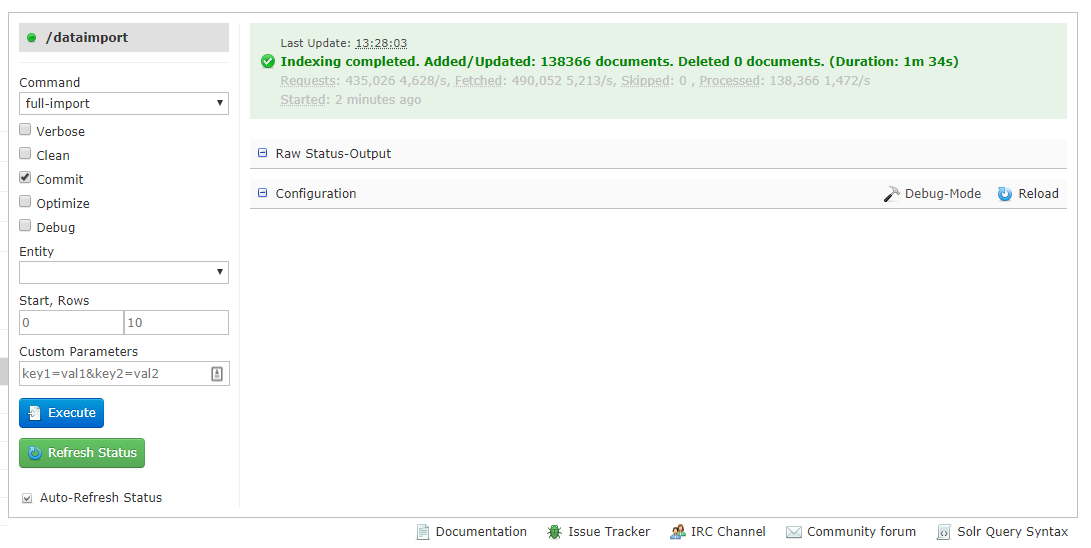
\includegraphics[width=1\linewidth]{images/solr_indexing_time.png}
	\caption{Indexierungsoberfläche mit Laufzeit.}
	\label{img:solrIndexTime}
\end{figure}

\subsection{Oberfläche}

Der Startseite des Solr-Systems bietet direkten Einblick in auf die Auslastung des Systems. Der Fehler-Log ist auch sehr einfach mit einem Klick zu erreichen. Um Statistiken zu dem aktuellen Core zu bekommen, kann dieser aus einen Drop-Down-Menu ausgewählt werden. Positiv anzumerken ist, dass es möglich ist das Schema direkt in der Weboberfläche zu modifizieren. Leider ist es nicht möglich, den DataImportHandler direkt zu verändern, ohne weitere Einstellungen im System vorzunehmen. Es gibt eine Möglichkeit Querys direkt über den Web-Client zu senden, was zum Testen und debuggen sehr nützlich ist. Auch bei der Indexierung kann ein Debug-Modus dazu geschaltet werden \ref{img:solrIndexTime}. Zudem gibt es die Möglichkeit die Konfigurationsdateien des Cores auf der Weboberfläche einzusehen, jedoch ist eine Editierung nicht möglich.
Es gibt keine Möglichkeit Updates direkt über die Weboberfläche einzuspielen, zudem ist die Seite auch nicht responsive geschrieben. 

\begin{figure}
	\centering
	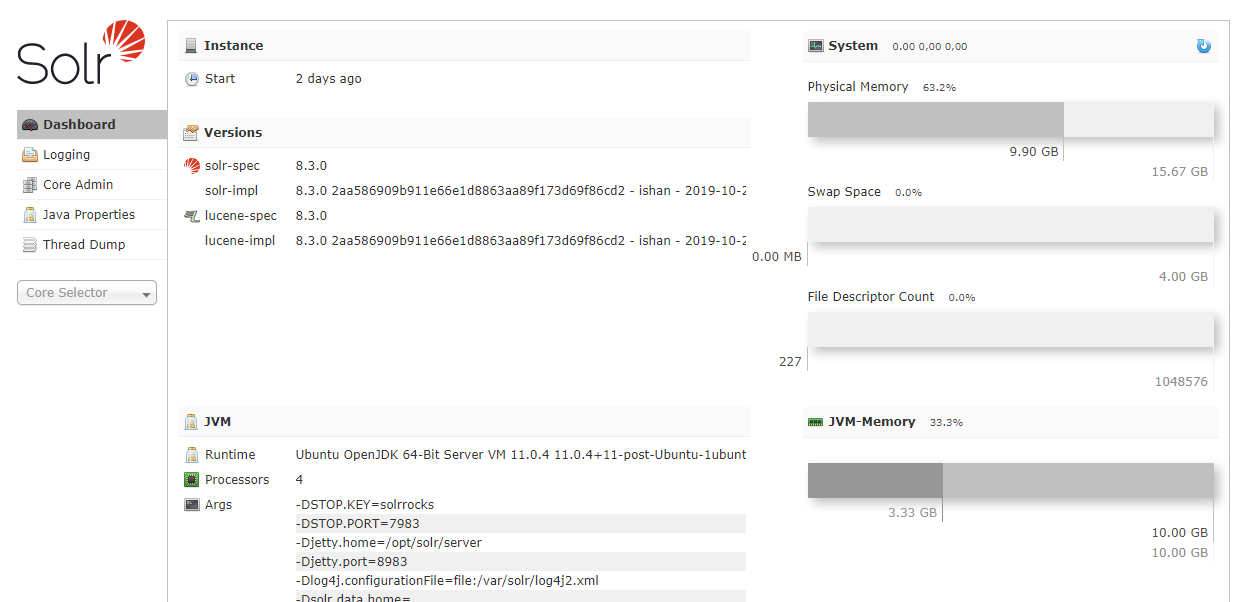
\includegraphics[width=1\linewidth]{images/solr_interface.png}
	\caption{Startseite der Weboberfläche von Solr.}
	\label{img:solrInterface}
\end{figure}


\subsection{Dokumentation}

Die Dokumentation war bei diesen kurzen Test meine Hauptquelle, die Installation ist dort sehr genau beschrieben. Positiv aufgefallen ist dabei vorallem die genaue Beschreibung der Systemanforderungen. Generell gibt es für alle Themen eine kleine Übersichtsseite, welche die grundlegenden Funktionen erklärt, ohne sich dabei in Details zu verlieren. 
Die Seite für den DataImportHandler hat anhand eines Beispiels gut die Struktur des Handlers abgebildet. Allerdings wäre ein Verweis, dass für die DataImportHandler-Attribute noch extra ein Solr-Schema-Attribut benötigt wird, schön gewesen. Dies habe ich erst durch einen Blog \cite{IqubalMustafaKaki.2016} herausgefunden und richtig verstanden. 
Die Dokumentation ist zum Reinlesen in die Grundlagen des Systems vollkommen ausreichend und bietet mit den Übersichtsseiten für die einzelnen Themen einen guten Startpunkt.

\subsection{Absetzen einer Anfrage und Integration in PHP}

Um nicht direkt mit der JSON-API arbeiten zu müssen, gibt es diverse Bibliotheken, die einige Arbeit abnehmen. Eine der größten ist hierbei Solarium, welches sich über Composer installieren lässt. Dies passt sehr gut zum Dietrich-Online Projekt, da auch dieses auf Composer aufbaut. Die Query ist herbei sehr einfach, da die Daten beim Import schon für diesen Query optimiert wurden.

\begin{lstlisting}[language=php, frame=single, label={lst:managedSchema}, 
  morekeywords={type,uninvertible,indexed,stored,field,multiValued, name}] 

  [...] # Imports and variable declarations

  $config = array(
      'endpoint' => array(
          'localhost' => array(
              'host' => '136.199.34.55',
              'port' => 8983,
              'core' => 'dietrich'
  )));
  $queryText = 'original_bezeichnung:S*';
  $solr = new Client($config);
  $query = $solr->createSelect();
  $query->setQuery($queryText);
  $query->setRows(2147483647); 
  [...] # Loop with Timer
  $resultSet = $solr->select($query);
  $count = $resultSet->count();
  [...] # Output Runtime
\end{lstlisting}

Interessant bei der Verbindung ist, dass die Anzahl der Zeilen die von Solr geladen werden, standardmäßig auf 10 limitiert sind. Erst mit setRows kann die Anzahl erhöht werden. Ich habe hierfür den maximalen Integer-Wert gewählt, um immer alle Ergebnisse zu bekommen. Um bei diesen Test nun einen guten Median-Wert zu erhalten, habe ich die Abfrage 100 mal laufen lassen. Dabei lieft die Abfrage durchschnittlich 1.01 Sekunden um die 15838 Ergebnisse herauszusuchen. Eine Vergleichtabelle, wie sich Solr dabei mit den anderen Suchmaschinen schlägt, finden Sie hier. !!VERGLEICH ANFÜGEN!!
